\chapter{Použité technologie}
\label{3-technologie}

Třetí kapitola stručně představuje jednotlivé technologie použité při tvorbě zásuvného modulu.

\section{QGIS}

\begin{figure}[H]
    \centering
      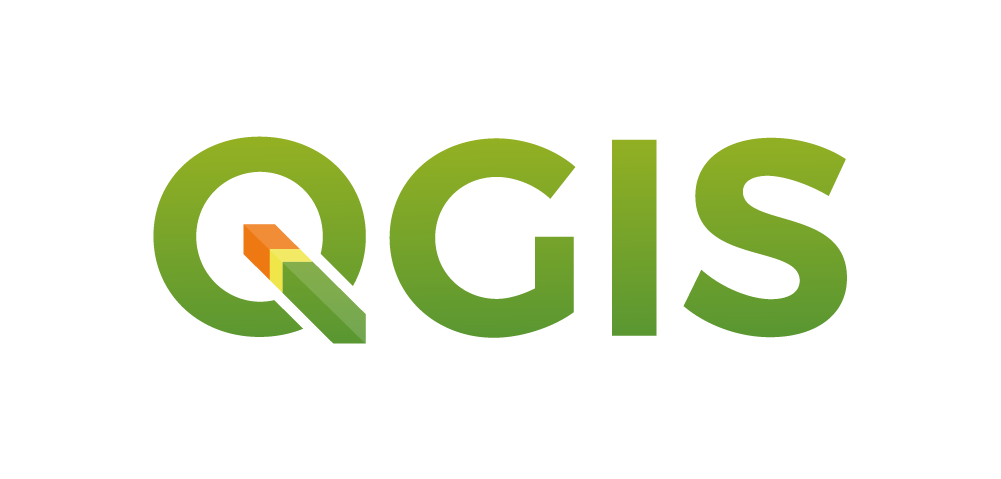
\includegraphics[width=200pt]{./pictures/qgis-logo.png}
      \caption[QGIS logo]{QGIS logo 
      (zdroj: \href{https://www.qgis.org/en/_downloads/qgis-logo.png}{QGIS})}
      \label{fig:qgis}
  \end{figure}

QGIS (dříve známý pod názvem Quantum GIS) je multiplatformní volně dostupný geografický informační systém (\zk{GIS}). Umožňuje uživateli prohlížet, vytvářet, analyzovat a editovat jak vektorová, tak rastrová prostorová data.

Vývoj započal v roce 2002 Gary Sherman, dnes ho spravuje skupina dobrovolníků a je vyvíjen pod hlavičkou Open Source Geospatial Foundation (\zk{OSGeo}). Hlavní myšlenkou při vzniku bylo vytvoření GIS softwaru dostupného zdarma každému vlastníkovi osobního počítače, na rozdíl od drahých komerčních softwarů. Ty ho ve všech aspektech sice většinou předčí, avšak pro běžného uživatele je QGIS zcela dostačující.

QGIS je vyvíjen v jazyku C++, jeho grafické rozhraní využívá knihovnu Qt. Je podporován na operačních systémech Microsoft Windows, Mac OS X, Linux a Unix, od roku 2014 existuje experimentální verze pro Android\footnote{http://www.qgis.org/en/site/forusers/download.html}. Základní funkcionalitu pomáhají rozšířit zásuvné moduly psané v jazyce Python nebo C++. Je propojen s dalšími open source GIS balíčky jako jsou např. GRASS GIS, PostGIS nebo MapServer. QGIS je uvolněn pod licencí GNU (\zk{GPL}) verze 2 a vyšší.

Komunita kolem QGIS aktivně podporuje své členy k přispívání a zlepšování softwaru - hlášením chyb, překládáním programu do dalších jazyků nebo snadným přístupem k tvorbě zásuvných modulů a jejich implementaci. 

% (1) http://www.qgis.org/en/site/forusers/download.html

\section{Python}

\begin{figure}[H]
    \centering
      
\includegraphics[width=150pt]{./pictures/python-logo-master-v3-TM.png}
      \caption[Python logo]{Python logo 
      (zdroj: \href{https://www.python.org/static/community_logos/python-logo-master-v3-TM.png}{Python.org})}
      \label{fig:python}
  \end{figure}
  
Python je vysokoúrovňový, interpretovaný programovací jazyk. Podporuje procedurálně i objektově orientované programování, je výkonný, zároveň má velmi jednoduchou a čistou syntax. V ostatních jazycích je odsazování řádků doporučeno z hlediska přehlednosti, u Pythonu je základním stavebním kamenem a je povinné. 

Guido van Rossum, autor první verze Pythonu vydané v roce 1991, se rozhodl vyřešit nedostatečnost jazyků, které byly používány v jeho zaměstnání, a napsat jazyk splňující jeho potřeby. Při vývoji se inspiroval především v jazycích ABC a Modula-3. Jednou ze snah bylo vytvoření jazyka otevřeného dalším rozšířením a propojením s jinými jazyky (např. C++). Dnes je Python vyvíjen jako open source projekt pod záštitou neziskové the Python Software Foundation (\zk{PSF}). Je distribuován pod licencí (\zk{PSF}), která je s (\zk{GPL}) kompatibilní. Je možné ho nainstalovat na běžné platformy jako Windows, Unix nebo Mac OS, pro Linux je většinou součástí základní instalace. Při vyvarování se systémově závislých funkcí je přenositelný mezi platformami bez jakýchkoli změn.

Python má široké využití, od jednoduchých programů po rozsáhlé aplikace. Právě pro tyto možnosti, univerzálnost, přehlednost kódu a síla z něj udělaly programovací jazyk, který je mezi začátečníky ve velké oblibě. Během krátké doby v něm funkční skript zvládne napsat každý. 
  
% (3) https://docs.python.org/3/faq/general.html#general-python-faq
  
\section{GDAL}  

Geospatial Data Abstraction Library (\zk{GDAL}) je knihovna určená pro čtení a zápis rastrových a vektorových geodat. Od verze GDAL 2.0 došlo k pevnějšímu propojení dvou původně oddělených knihoven - GDAL, pracující s rastrovými daty, a OGR, zpracovávající data vektorová.

Do verze 1.3.2 byla vyvíjena Frankem Warmerdamem. Další údržba byla převedena na GDAL/OGR Project Management Committee, která je součástí \zk{OSGeo} Foundation. 

GDAL/OGR je napsána v jazyce ANSI C a C++ a lze ji použít na operačních systémech Linux, Solaris, Mac OS X a Microsoft Windows. Knihovna GDAL je vydávána pod licencí X/MIT. (4) Pro projekce a transformace využívá knihovnu PROJ.4. V květnu 2017 byla vydána zatím poslední verze GDAL 2.2.0. (4)

Díky rozsáhlému množství funkcionalit je využívána v komerční i nekomerční sféře a v oblasti GIS patří mezi hlavní free software projekty.

% (4) http://www.gdal.org/ (hlavní strana + FAQ)

\section{Qt Project}

\begin{figure}[H]
    \centering
      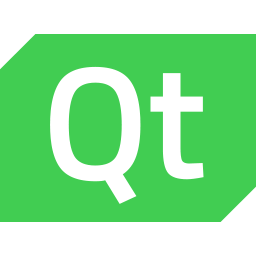
\includegraphics[width=100pt]{./pictures/qt_logo_green_256x256px.png}
      \caption[Qt Project logo]{Qt Project logo 
      (zdroj: \href{http://brand.qt.io/downloads/}{qt.io})}
      \label{fig:qt}
  \end{figure}

Qt je framework\footnote{multiplatformní aplikační rámec} knihoven a nástrojů, jenž je široce využíván pro tvorbu multiplatformních aplikací a grafických uživatelských rozhraní. Svou oblibu si vysloužil právě funkčností na různých softwarových i hardwarových platformách, kdy je třeba do kódu zavést jen pár změn nebo ho neupravovat vůbec. Další výhodou je velmi dobře zpracovaná dokumentace.

Qt je založen na jazyku C++. Na vývoji Qt se v současnosti podílejí dvě společnosti - The Qt Company a Qt Project, z nichž druhá jmenovaná následuje politiku otevřených dat. Qt je tedy dostupný jak pod komerční licencí, tak pod open source licencemi GNU \zk{GPL} 2.0, GNU \zk{GPL} 3.0 a \zk{LGPL} 3.0. Poslední verzí vydanou před květnem 2017 byla verze Qt 5.8. (5)

% zmínit Qt Designer
% (5) https://www.qt.io/company/

\subsection{PyQt}
Qt je sice psán v jazyce C++, ale existuje mnoho rozhraní pro programování aplikací (\zk{API}) umožňujících propojení s dalšími programovacími jazyky. Pro Python patří mezi nejoblíbenější PyQt a PySide.

Správa a vývoj PyQt spadá pod firmu Riverbank Computing Limited. PyQt je dostupný pod podobnou licencí jako Qt, tedy GNU \zk{GPL} 2.0, GNU \zk{GPL} 3.0 a komerční licencí.

% (6) https://wiki.python.org/moin/PyQt

